% Options for packages loaded elsewhere
% Options for packages loaded elsewhere
\PassOptionsToPackage{unicode}{hyperref}
\PassOptionsToPackage{hyphens}{url}
\PassOptionsToPackage{dvipsnames,svgnames,x11names}{xcolor}
%
\documentclass[
  spanish,
  a4paper,
  oneside]{scrbook}
\usepackage{xcolor}
\usepackage[top=25mm,bottom=25mm,left=30mm,right=20mm]{geometry}
\usepackage{amsmath,amssymb}
\setcounter{secnumdepth}{5}
\usepackage{iftex}
\ifPDFTeX
  \usepackage[T1]{fontenc}
  \usepackage[utf8]{inputenc}
  \usepackage{textcomp} % provide euro and other symbols
\else % if luatex or xetex
  \usepackage{unicode-math} % this also loads fontspec
  \defaultfontfeatures{Scale=MatchLowercase}
  \defaultfontfeatures[\rmfamily]{Ligatures=TeX,Scale=1}
\fi
\usepackage{lmodern}
\ifPDFTeX\else
  % xetex/luatex font selection
\fi
% Use upquote if available, for straight quotes in verbatim environments
\IfFileExists{upquote.sty}{\usepackage{upquote}}{}
\IfFileExists{microtype.sty}{% use microtype if available
  \usepackage[]{microtype}
  \UseMicrotypeSet[protrusion]{basicmath} % disable protrusion for tt fonts
}{}
\makeatletter
\@ifundefined{KOMAClassName}{% if non-KOMA class
  \IfFileExists{parskip.sty}{%
    \usepackage{parskip}
  }{% else
    \setlength{\parindent}{0pt}
    \setlength{\parskip}{6pt plus 2pt minus 1pt}}
}{% if KOMA class
  \KOMAoptions{parskip=half}}
\makeatother
% Make \paragraph and \subparagraph free-standing
\makeatletter
\ifx\paragraph\undefined\else
  \let\oldparagraph\paragraph
  \renewcommand{\paragraph}{
    \@ifstar
      \xxxParagraphStar
      \xxxParagraphNoStar
  }
  \newcommand{\xxxParagraphStar}[1]{\oldparagraph*{#1}\mbox{}}
  \newcommand{\xxxParagraphNoStar}[1]{\oldparagraph{#1}\mbox{}}
\fi
\ifx\subparagraph\undefined\else
  \let\oldsubparagraph\subparagraph
  \renewcommand{\subparagraph}{
    \@ifstar
      \xxxSubParagraphStar
      \xxxSubParagraphNoStar
  }
  \newcommand{\xxxSubParagraphStar}[1]{\oldsubparagraph*{#1}\mbox{}}
  \newcommand{\xxxSubParagraphNoStar}[1]{\oldsubparagraph{#1}\mbox{}}
\fi
\makeatother

\usepackage{color}
\usepackage{fancyvrb}
\newcommand{\VerbBar}{|}
\newcommand{\VERB}{\Verb[commandchars=\\\{\}]}
\DefineVerbatimEnvironment{Highlighting}{Verbatim}{commandchars=\\\{\}}
% Add ',fontsize=\small' for more characters per line
\usepackage{framed}
\definecolor{shadecolor}{RGB}{241,243,245}
\newenvironment{Shaded}{\begin{snugshade}}{\end{snugshade}}
\newcommand{\AlertTok}[1]{\textcolor[rgb]{0.68,0.00,0.00}{#1}}
\newcommand{\AnnotationTok}[1]{\textcolor[rgb]{0.37,0.37,0.37}{#1}}
\newcommand{\AttributeTok}[1]{\textcolor[rgb]{0.40,0.45,0.13}{#1}}
\newcommand{\BaseNTok}[1]{\textcolor[rgb]{0.68,0.00,0.00}{#1}}
\newcommand{\BuiltInTok}[1]{\textcolor[rgb]{0.00,0.23,0.31}{#1}}
\newcommand{\CharTok}[1]{\textcolor[rgb]{0.13,0.47,0.30}{#1}}
\newcommand{\CommentTok}[1]{\textcolor[rgb]{0.37,0.37,0.37}{#1}}
\newcommand{\CommentVarTok}[1]{\textcolor[rgb]{0.37,0.37,0.37}{\textit{#1}}}
\newcommand{\ConstantTok}[1]{\textcolor[rgb]{0.56,0.35,0.01}{#1}}
\newcommand{\ControlFlowTok}[1]{\textcolor[rgb]{0.00,0.23,0.31}{\textbf{#1}}}
\newcommand{\DataTypeTok}[1]{\textcolor[rgb]{0.68,0.00,0.00}{#1}}
\newcommand{\DecValTok}[1]{\textcolor[rgb]{0.68,0.00,0.00}{#1}}
\newcommand{\DocumentationTok}[1]{\textcolor[rgb]{0.37,0.37,0.37}{\textit{#1}}}
\newcommand{\ErrorTok}[1]{\textcolor[rgb]{0.68,0.00,0.00}{#1}}
\newcommand{\ExtensionTok}[1]{\textcolor[rgb]{0.00,0.23,0.31}{#1}}
\newcommand{\FloatTok}[1]{\textcolor[rgb]{0.68,0.00,0.00}{#1}}
\newcommand{\FunctionTok}[1]{\textcolor[rgb]{0.28,0.35,0.67}{#1}}
\newcommand{\ImportTok}[1]{\textcolor[rgb]{0.00,0.46,0.62}{#1}}
\newcommand{\InformationTok}[1]{\textcolor[rgb]{0.37,0.37,0.37}{#1}}
\newcommand{\KeywordTok}[1]{\textcolor[rgb]{0.00,0.23,0.31}{\textbf{#1}}}
\newcommand{\NormalTok}[1]{\textcolor[rgb]{0.00,0.23,0.31}{#1}}
\newcommand{\OperatorTok}[1]{\textcolor[rgb]{0.37,0.37,0.37}{#1}}
\newcommand{\OtherTok}[1]{\textcolor[rgb]{0.00,0.23,0.31}{#1}}
\newcommand{\PreprocessorTok}[1]{\textcolor[rgb]{0.68,0.00,0.00}{#1}}
\newcommand{\RegionMarkerTok}[1]{\textcolor[rgb]{0.00,0.23,0.31}{#1}}
\newcommand{\SpecialCharTok}[1]{\textcolor[rgb]{0.37,0.37,0.37}{#1}}
\newcommand{\SpecialStringTok}[1]{\textcolor[rgb]{0.13,0.47,0.30}{#1}}
\newcommand{\StringTok}[1]{\textcolor[rgb]{0.13,0.47,0.30}{#1}}
\newcommand{\VariableTok}[1]{\textcolor[rgb]{0.07,0.07,0.07}{#1}}
\newcommand{\VerbatimStringTok}[1]{\textcolor[rgb]{0.13,0.47,0.30}{#1}}
\newcommand{\WarningTok}[1]{\textcolor[rgb]{0.37,0.37,0.37}{\textit{#1}}}

\usepackage{longtable,booktabs,array}
\newcounter{none} % for unnumbered tables
\usepackage{calc} % for calculating minipage widths
% Correct order of tables after \paragraph or \subparagraph
\usepackage{etoolbox}
\makeatletter
\patchcmd\longtable{\par}{\if@noskipsec\mbox{}\fi\par}{}{}
\makeatother
% Allow footnotes in longtable head/foot
\IfFileExists{footnotehyper.sty}{\usepackage{footnotehyper}}{\usepackage{footnote}}
\makesavenoteenv{longtable}
\usepackage{graphicx}
\makeatletter
\newsavebox\pandoc@box
\newcommand*\pandocbounded[1]{% scales image to fit in text height/width
  \sbox\pandoc@box{#1}%
  \Gscale@div\@tempa{\textheight}{\dimexpr\ht\pandoc@box+\dp\pandoc@box\relax}%
  \Gscale@div\@tempb{\linewidth}{\wd\pandoc@box}%
  \ifdim\@tempb\p@<\@tempa\p@\let\@tempa\@tempb\fi% select the smaller of both
  \ifdim\@tempa\p@<\p@\scalebox{\@tempa}{\usebox\pandoc@box}%
  \else\usebox{\pandoc@box}%
  \fi%
}
% Set default figure placement to htbp
\def\fps@figure{htbp}
\makeatother


% definitions for citeproc citations
\NewDocumentCommand\citeproctext{}{}
\NewDocumentCommand\citeproc{mm}{%
  \begingroup\def\citeproctext{#2}\cite{#1}\endgroup}
\makeatletter
 % allow citations to break across lines
 \let\@cite@ofmt\@firstofone
 % avoid brackets around text for \cite:
 \def\@biblabel#1{}
 \def\@cite#1#2{{#1\if@tempswa , #2\fi}}
\makeatother
\newlength{\cslhangindent}
\setlength{\cslhangindent}{1.5em}
\newlength{\csllabelwidth}
\setlength{\csllabelwidth}{3em}
\newenvironment{CSLReferences}[2] % #1 hanging-indent, #2 entry-spacing
 {\begin{list}{}{%
  \setlength{\itemindent}{0pt}
  \setlength{\leftmargin}{0pt}
  \setlength{\parsep}{0pt}
  % turn on hanging indent if param 1 is 1
  \ifodd #1
   \setlength{\leftmargin}{\cslhangindent}
   \setlength{\itemindent}{-1\cslhangindent}
  \fi
  % set entry spacing
  \setlength{\itemsep}{#2\baselineskip}}}
 {\end{list}}
\usepackage{calc}
\newcommand{\CSLBlock}[1]{\hfill\break\parbox[t]{\linewidth}{\strut\ignorespaces#1\strut}}
\newcommand{\CSLLeftMargin}[1]{\parbox[t]{\csllabelwidth}{\strut#1\strut}}
\newcommand{\CSLRightInline}[1]{\parbox[t]{\linewidth - \csllabelwidth}{\strut#1\strut}}
\newcommand{\CSLIndent}[1]{\hspace{\cslhangindent}#1}

\ifLuaTeX
\usepackage[bidi=basic,shorthands=off]{babel}
\else
\usepackage[bidi=default,shorthands=off]{babel}
\fi
\ifLuaTeX
  \usepackage{selnolig} % disable illegal ligatures
\fi


\setlength{\emergencystretch}{3em} % prevent overfull lines

\providecommand{\tightlist}{%
  \setlength{\itemsep}{0pt}\setlength{\parskip}{0pt}}



 


\AtBeginDocument{\hypersetup{linkcolor=black}}
% ---------- Paquetes tipograficos y microajustes ----------
\usepackage{microtype}        % mejor interletrado y justificado
\usepackage{csquotes}         % comillas tipograficas
\usepackage{iftex}
\ifPDFTeX\else
  % Seleccion de fuentes solo cuando XeTeX/LuaTeX esta disponible.
  \IfFontExistsTF{TeX Gyre Termes}{
    \setmainfont{TeX Gyre Termes}
  }{
    \IfFontExistsTF{Latin Modern Roman}{\setmainfont{Latin Modern Roman}}{}
  }
  \IfFontExistsTF{TeX Gyre Heros}{
    \setsansfont{TeX Gyre Heros}
  }{
    \IfFontExistsTF{Latin Modern Sans}{\setsansfont{Latin Modern Sans}}{}
  }
  \IfFontExistsTF{TeX Gyre Cursor}{
    \setmonofont{TeX Gyre Cursor}
  }{
    \IfFontExistsTF{Latin Modern Mono}{\setmonofont{Latin Modern Mono}}{}
  }
\fi
\usepackage{enumitem}         % listas compactas
\setlist{itemsep=.2em, topsep=.2em}

% ---------- KOMA-Script: estilo de titulos y espaciado ----------
\KOMAoptions{
  headings=big,
  parskip=half,
  fontsize=12pt,
  appendixprefix=true
}
\setlength{\parindent}{1.5em}
\setlength{\parskip}{0.6em}
\usepackage{indentfirst}
\usepackage{setspace}         % Control del interlineado del documento
\setstretch{1.5}

% ---------- Encabezados y pies (scrlayer-scrpage) ----------
\usepackage[automark,headsepline]{scrlayer-scrpage}
\clearpairofpagestyles
\automark[chapter]{chapter}
\ihead{\pagemark}
\ohead{\itshape\headmark}
\setheadsepline{0.4pt}
\renewcommand*{\chaptermarkformat}{}
\renewcommand*{\chapterpagestyle}{scrheadings}
\pagestyle{scrheadings}
\makeatletter
\let\ps@plain\ps@scrheadings
\makeatother
\cfoot{}

% ---------- Hipervinculos mas sobrios ----------
\usepackage{hyperref}
\hypersetup{
  colorlinks=true,
  linkcolor=black,
  citecolor=[rgb]{0.05,0.2,0.5},
  urlcolor=[rgb]{0.05,0.2,0.5},
  pdfauthor={\@author},
  pdftitle={\@title}
}

% ---------- Leyendas de figuras/tablas ----------
\usepackage[labelfont=bf,textfont=it]{caption}
\captionsetup{
  skip=8pt
}

% ---------- Tabla de contenidos ----------
\KOMAoptions{toc=graduated}
\RedeclareSectionCommand[tocnumwidth=3em]{chapter}
\RedeclareSectionCommand[tocindent=3.25em,tocnumwidth=2.8em]{section}
\RedeclareSectionCommand[tocindent=6.5em,tocnumwidth=2.5em]{subsection}
\makeatletter
\newcommand*{\tocdotfill}{\leavevmode\leaders\hbox to .6em{\hss.\hss}\hfill}
\makeatother
\RedeclareSectionCommand[toclinefill=\tocdotfill]{chapter}
\RedeclareSectionCommand[toclinefill=\tocdotfill]{section}
\RedeclareSectionCommand[toclinefill=\tocdotfill]{subsection}
\renewcommand*{\contentsname}{Tabla de contenido}
\setkomafont{chapterentry}{\normalfont}
\setkomafont{chapterentrypagenumber}{\normalfont}

% ---------- Viudas/Huerfanas y cortes de pagina ----------
\clubpenalty=10000
\widowpenalty=10000
\displaywidowpenalty=10000

% ---------- Entorno abstract para scrbook ----------
\providecommand{\abstractname}{Resumen}
\makeatletter
\@ifundefined{abstract}{
  \newenvironment{abstract}{
    \cleardoublepage
    \thispagestyle{plain}
    \null\vfill
    \begin{center}
      {\bfseries\Large \abstractname\par}
    \end{center}\vspace{1em}
    \begingroup
  }{
    \par\endgroup
    \vfill\null
    \cleardoublepage
  }
}{}
\makeatother

% ---------- Soporte de subtitulo desde YAML ----------
\makeatletter
\providecommand{\subtitle}[1]{\gdef\@subtitle{#1}}
\providecommand{\@subtitle}{}
\makeatother

\makeatletter
\newcommand{\facso@iflist}[4]{%
  \begingroup
    \def\addvspace##1{}%
    \def\numberline##1{##1}%
    \def\facso@target{#2}%
    \newcount\facso@entrycount
    \facso@entrycount=0\relax
    \long\def\contentsline##1##2##3{%
      \def\facso@this{##1}%
      \ifx\facso@this\facso@target
        \advance\facso@entrycount\@ne
      \fi
    }%
    \InputIfFileExists{\jobname.#1}{}{}%
  \endgroup
  \ifnum\facso@entrycount>0\relax
    #3%
  \else
    #4%
  \fi}
\renewcommand{\listoffigures}{%
  \facso@iflist{lof}{figure}{%
    \cleardoublepage
    \phantomsection
    \addchap*{Listado de Figuras}%
    \thispagestyle{scrheadings}%
    \markboth{Listado de Figuras}{Listado de Figuras}%
    \addcontentsline{toc}{chapter}{Listado de Figuras}%
    \@starttoc{lof}%
    \cleardoublepage
    \automark[chapter]{chapter}%
  }{}}
\renewcommand{\listoftables}{%
  \facso@iflist{lot}{table}{%
    \cleardoublepage
    \phantomsection
    \addchap*{Listado de Tablas}%
    \thispagestyle{scrheadings}%
    \markboth{Listado de Tablas}{Listado de Tablas}%
    \addcontentsline{toc}{chapter}{Listado de Tablas}%
    \@starttoc{lot}%
    \cleardoublepage
    \automark[chapter]{chapter}%
  }{}}
\makeatother

% --- Desactivar portada y abstract automaticos de Pandoc (PDF) ---
\AtBeginDocument{\let\maketitle\relax}
\renewenvironment{abstract}{}{}
\providecommand{\appendixname}{}
\providecommand{\appendixtocname}{}
\providecommand{\appendixpagename}{}
\renewcommand*{\appendixname}{Anexo}
\renewcommand*{\appendixtocname}{Anexos}
\renewcommand*{\appendixpagename}{Anexos}
\usepackage{booktabs}
\usepackage{caption}
\usepackage{longtable}
\usepackage{colortbl}
\usepackage{array}
\usepackage{anyfontsize}
\usepackage{multirow}
\makeatletter
\@ifpackageloaded{bookmark}{}{\usepackage{bookmark}}
\makeatother
\makeatletter
\@ifpackageloaded{caption}{}{\usepackage{caption}}
\AtBeginDocument{%
\ifdefined\contentsname
  \renewcommand*\contentsname{Tabla de contenidos}
\else
  \newcommand\contentsname{Tabla de contenidos}
\fi
\ifdefined\listfigurename
  \renewcommand*\listfigurename{Listado de Figuras}
\else
  \newcommand\listfigurename{Listado de Figuras}
\fi
\ifdefined\listtablename
  \renewcommand*\listtablename{Listado de Tablas}
\else
  \newcommand\listtablename{Listado de Tablas}
\fi
\ifdefined\figurename
  \renewcommand*\figurename{Lista de figuras}
\else
  \newcommand\figurename{Lista de figuras}
\fi
\ifdefined\tablename
  \renewcommand*\tablename{Lista de tablas}
\else
  \newcommand\tablename{Lista de tablas}
\fi
}
\@ifpackageloaded{float}{}{\usepackage{float}}
\floatstyle{ruled}
\@ifundefined{c@chapter}{\newfloat{codelisting}{h}{lop}}{\newfloat{codelisting}{h}{lop}[chapter]}
\floatname{codelisting}{Listado}
\newcommand*\listoflistings{\listof{codelisting}{Listado de Listados}}
\makeatother
\makeatletter
\makeatother
\makeatletter
\@ifpackageloaded{caption}{}{\usepackage{caption}}
\@ifpackageloaded{subcaption}{}{\usepackage{subcaption}}
\makeatother
\usepackage{bookmark}
\IfFileExists{xurl.sty}{\usepackage{xurl}}{} % add URL line breaks if available
\urlstyle{same}
\hypersetup{
  pdftitle={Título del trabajo},
  pdfauthor={Nicolás Outerbridge; Vicente Rojas},
  pdflang={es},
  colorlinks=true,
  linkcolor={Maroon},
  filecolor={Maroon},
  citecolor={Blue},
  urlcolor={Blue},
  pdfcreator={LaTeX via pandoc}}


\title{Título del trabajo}
\usepackage{etoolbox}
\makeatletter
\providecommand{\subtitle}[1]{% add subtitle to \maketitle
  \apptocmd{\@title}{\par {\large #1 \par}}{}{}
}
\makeatother
\subtitle{Trabajo final}
\author{Nicolás Outerbridge \and Vicente Rojas}
\date{27 de junio de 2026}
\begin{document}
\frontmatter
\maketitle

% --- title-pdf.tex personalizado para portada formal ---
\makeatletter
\providecommand{\subtitle}[1]{\gdef\@subtitle{#1}}
\providecommand{\@subtitle}{}
\providecommand{\frontmattercontext}{}
\providecommand{\advisorname}{}
\providecommand{\advisorlabel}{FACSO}
\providecommand{\frontmatterlocation}{}
\InputIfFileExists{includes/cover-config.tex}{}{}

\newcommand{\PrintTitle}{%
  {\sffamily\bfseries\fontsize{24pt}{28pt}\selectfont \@title\par}%
}
\newcommand{\PrintSubtitle}{%
  \begingroup
  \edef\temp{\detokenize{\@subtitle}}%
  \ifx\temp\empty\relax
    % sin subtitulo
  \else
    {\sffamily\bfseries\large \@subtitle\par}%
  \fi
  \endgroup
}
\newcommand{\PrintAuthor}{%
  \begingroup
  \def\and{\\}% \and separa autores con salto de linea (en vez del \and de \maketitle estandar, que requiere una tabla abierta)
  {\Large\bfseries \@author\par}%
  \endgroup
}
\newcommand{\PrintDate}{%
  {\small \@date\par}%
}
\makeatother

\begin{titlepage}
\thispagestyle{empty}
\begin{center}
\vspace*{10mm}

% Logo o imagen institucional

\includegraphics[width=0.35\textwidth]{assets/cover.png}\par
\vspace{12mm}

% Titulo y subtitulo
\PrintTitle
\vspace{6mm}
\PrintSubtitle

\vspace{22mm}
\begingroup
\edef\temp{\detokenize{\frontmattercontext}}%
\ifx\temp\empty\relax
  % sin contexto adicional
\else
  {\normalsize \frontmattercontext\par}
\fi
\endgroup

\vspace{18mm}
\PrintAuthor

\vspace{16mm}
\begingroup
\edef\temp{\detokenize{\advisorname}}%
\ifx\temp\empty\relax
  % sin tutor
\else
  \rule{0.45\textwidth}{0.4pt}\par
  {\small \advisorlabel\ \advisorname\par}
\fi
\endgroup

\vfill
\begingroup
\edef\temp{\detokenize{\frontmatterlocation}}%
\ifx\temp\empty\relax
  % sin ubicacion
\else
  {\small \frontmatterlocation\par}
\fi
\endgroup
\PrintDate

\end{center}
\end{titlepage}

% Preliminares (numeros romanos) y estilo simple
\frontmatter
\pagestyle{scrheadings}

\setcounter{tocdepth}{2} % (o 1/3 segun prefieras)
\tableofcontents
\listoffigures
\listoftables


\mainmatter
\bookmarksetup{startatroot}

\chapter*{Abstract}\label{abstract}
\addcontentsline{toc}{chapter}{Abstract}

\markboth{Abstract}{Abstract}

\small\textbf{Palabras clave:} Ciencia Social Abierta \normalsize

\bookmarksetup{startatroot}

\chapter{Introducción}\label{introducciuxf3n}

La confianza en las instituciones del Estado figura en el debate
sociológico contemporáneo como un indicador crítico para evaluar la
estabilidad democrática y la legitimidad de los regímenes políticos
{«({PDF}) {The Essentials} of {Social Cohesion}»}
(\citeproc{ref-_essentials_2017}{2017}). Tradicionalmente entendida como
el grado de certidumbre y satisfacción que la ciudadanía deposita en el
desempeño gubernamental y en la probidad de sus organizaciones
(\citeproc{ref-han_trust_2021}{Han et~al., 2021}), el concepto opera
como una valoración implícita de que las agencias estatales orientan sus
prerrogativas hacia la consecución del bien común y el resguardo de los
valores compartidos (\citeproc{ref-_cohesion_2022}{\emph{{Cohesión
social en Chile en tiempos de cambio}}, 2022}). En términos funcionales,
la literatura especializada destaca que la confianza es un recurso
bidireccional indispensable: para el aparato estatal, constituye una
fuente de poder que fomenta la obediencia voluntaria de las normas y
reduce los costos de coerción
(\citeproc{ref-ministeriodedesarrollosocialyfamilia_informe_2020}{Ministerio
de Desarrollo Social y Familia, 2020}); mientras que para los
ciudadanos, actúa como un mecanismo de simplificación cognitiva que
mitiga la necesidad de fiscalizar exhaustivamente cada praxis
gubernamental. No obstante, este recurso no reviste un carácter
estático, sino que se reconfigura dinámicamente a partir de la
estratificación socioeconómica de la población. La evidencia
internacional sugiere que la clase social, tanto en sus dimensiones
objetivas como subjetivas, constituye el principal predictor de la
confianza institucional, superando incluso el impacto de la desigualdad
agregada de ingresos (\citeproc{ref-kim_social_2021}{Kim et~al., 2021}).
Esto responde a que la heterogeneidad estructural del mercado laboral y
las distintas posiciones de clase configuran valoraciones asimétricas
respecto a la eficacia del Estado, observándose que los estratos dotados
de mayor capital económico y cultural tienden a evaluar el desempeño de
sus líderes bajo estándares normativos considerablemente más estrictos y
críticos (\citeproc{ref-kim_social_2021}{Kim et~al., 2021};
\citeproc{ref-molina_repensando_2022}{Molina \& Alfageme, 2022}). En el
escenario chileno actual, este fenómeno adquiere una urgencia empírica
sin precedentes. Tras enfrentar \emph{shocks} político-sociales y
sanitarios de gran envergadura ---tales como el estallido social de 2019
y las repercusiones de la pandemia por COVID-19---, el país ha
experimentado una contracción drástica de su capital institucional. Los
organismos fundamentales del régimen político chileno, tales como el
Congreso Nacional, el Ejecutivo y los partidos políticos, exhiben hoy
índices de confianza críticamente exiguos, situándose de manera
persistente por debajo del umbral del 5\%
(\citeproc{ref-ministeriodedesarrollosocialyfamilia_informe_2020}{Ministerio
de Desarrollo Social y Familia, 2020}). Esta erosión sistémica evidencia
que cuando el aparato estatal se percibe como incapaz de proveer
soluciones oportunas, eficaces y dignas a las demandas ciudadanas, el
tejido que vincula formalmente a la sociedad con el Estado se fractura
de forma severa (\citeproc{ref-han_trust_2021}{Han et~al., 2021};
\citeproc{ref-__cohesion_2022}{\textbf{\_\_cohesion\_2022?}}). Frente a
este diagnóstico de crisis y distanciamiento, el presente estudio tiene
por objetivo analizar el impacto de la clase social sobre la confianza
en las instituciones a lo largo del periodo 2016-2023, contemplando
algunas variabels de relevancia teorica como el nivel educativo y la
coherte generacional utilizando los datos del Estudio Longitudinal
Social de Chile (ELSOC). Esta investigación examina de qué manera las
diversas posiciones en la estructura social moldean y condicionan las
trayectorias temporales de la confianza institucional en una sociedad
marcada por la incertidumbre y la erosión de sus bases de legitimidad.

\bookmarksetup{startatroot}

\chapter{Antecedentes}\label{antecedentes}

La confianza en las instituciones se define como el grado de certidumbre
y satisfacción que la ciudadanía deposita en el desempeño gubernamental
y en la credibilidad de sus organizaciones
(\citeproc{ref-_confianza_2024}{{«{La confianza en las instituciones
públicas de Chile}»}, 2024}; \citeproc{ref-han2021}{\textbf{han2021?}}).
Teóricamente, este constructo representa el núcleo de la cohesión social
vertical, articulando el vínculo jerárquico entre el individuo y el
Estado (\citeproc{ref-chan_charting_2006}{Chan \& Chan, 2006};
\citeproc{ref-ministeriodedesarrollosocialyfamilia_informe_2020}{Ministerio
de Desarrollo Social y Familia, 2020}). Para {«({PDF}) {The Essentials}
of {Social Cohesion}»} (\citeproc{ref-_essentials_2017}{2017}), la
confianza es un elemento constitutivo esencial de la convivencia
colectiva, pues actúa como un recurso moral que reduce los costos de
gobernanza e incentiva la obediencia voluntaria de las normas.

Como ``pegamento social'', la confianza institucional es fundamental
para la estabilidad democrática, el crecimiento económico y el bienestar
de la población (\citeproc{ref-kim_social_2021}{Kim et~al., 2021}). Sin
embargo, a diferencia de la confianza interpersonal (dimensión
horizontal), la confianza en las instituciones es un fenómeno más
abstracto que depende de la percepción de legitimidad y de la capacidad
del sistema para representar valores compartidos
(\citeproc{ref-_cohesion_2022}{\emph{{Cohesión social en Chile en
tiempos de cambio}}, 2022}; \citeproc{ref-_essentials_2017}{{«({PDF})
{The Essentials} of {Social Cohesion}»}, 2017}).

En la última década, Chile ha experimentado un deterioro crítico en sus
índices de confianza pública. Según el informe de la OCDE (2024), solo
el 30\% de los chilenos manifiesta una confianza alta o moderadamente
alta en su gobierno nacional, una cifra significativamente menor al
promedio de los países miembros (39\%). Esta desafección es aún más
pronunciada en instituciones clave como el Congreso Nacional (19\%) y
los partidos políticos (14\%), lo que refleja una fractura profunda en
la legitimidad del sistema representativo
(\citeproc{ref-_confianza_2024}{{«{La confianza en las instituciones
públicas de Chile}»}, 2024}). La literatura identifica que esta erosión
se ha visto catalizada por shocks de contexto de gran magnitud: el
estallido social de 2019 y la pandemia del COVID-19
(\citeproc{ref-_cohesion_2022}{\emph{{Cohesión social en Chile en
tiempos de cambio}}, 2022}). Estos eventos actuaron como disrupciones
que pusieron a prueba la capacidad de respuesta del Estado. Cuando las
instituciones no logran proveer soluciones eficaces y dignas ante
situaciones de crisis, la confianza vertical se debilita de forma
sistémica, comprometiendo el contrato social
(\citeproc{ref-ministeriodedesarrollosocialyfamilia_informe_2020}{Ministerio
de Desarrollo Social y Familia, 2020};
\citeproc{ref-han2021}{\textbf{han2021?}}).

La confianza institucional no es un rasgo estático, sino que se
reconfigura según factores estructurales y de desempeño:

Integridad y Corrupción: La percepción de que las instituciones sirven
al interés público y la ausencia de corrupción son los predictores más
fuertes de la confianza (\citeproc{ref-_confianza_2024}{{«{La confianza
en las instituciones públicas de Chile}»}, 2024}). En Chile, la sospecha
de corrupción erosiona de raíz la legitimidad del vínculo jerárquico
sociedad-Estado
(\citeproc{ref-ministeriodedesarrollosocialyfamilia_informe_2020}{Ministerio
de Desarrollo Social y Familia, 2020}).

Clase Social y Educación: Kim et al. (\citeproc{ref-kim_social_2021}{Kim
et~al., 2021}) sugieren que los individuos con mayor capital cultural
(educación) tienden a evaluar a sus líderes con estándares más
exigentes, lo que puede derivar en una menor confianza. No obstante, en
América Latina, la heterogeneidad estructural y la exclusión de los
beneficios del desarrollo provocan que las clases trabajadoras manuales
presenten los niveles más bajos de adhesión al pacto social
(\citeproc{ref-molina_repensando_2022}{Molina \& Alfageme, 2022}).

Fractura Generacional: Existe un abismo etario creciente. Los grupos más
jóvenes, específicamente la Generación Z, exhiben niveles de confianza
sistemáticamente menores y un alejamiento del orden institucional en
comparación con las generaciones antiguas
(\citeproc{ref-diazsarmiento_entendiendo_2017}{Díaz Sarmiento et~al.,
2017}; \citeproc{ref-_confianza_2024}{{«{La confianza en las
instituciones públicas de Chile}»}, 2024}).

Sentido de Pertenencia: Existe un debilitamiento del vínculo
comunitario. Los altos niveles de desigualdad y la percepción de
discriminación actúan como fracturas del sentido de pertenencia en
Chile, fomentando la priorización del estatus económico personal por
sobre el destino compartido y mermando sistemáticamente la confianza en
las instituciones públicas (\citeproc{ref-_confianza_2024}{{«{La
confianza en las instituciones públicas de Chile}»}, 2024}).

\bookmarksetup{startatroot}

\chapter{Hipótesis}\label{hipuxf3tesis}

\section{Especificación del Modelo e Hipótesis de
Investigación}\label{especificaciuxf3n-del-modelo-e-hipuxf3tesis-de-investigaciuxf3n}

\subsection{Modelo de Regresión Multinivel
Longitudinal}\label{modelo-de-regresiuxf3n-multinivel-longitudinal}

\[
\begin{aligned}
c_{05_{ti}} = \gamma_{00} 
&+ \gamma_{10}\text{c38}_{i} + \gamma_{20}\text{edad}_{i} + \gamma_{30}\text{trato}_{i} + \gamma_{40}\text{c15}_{i} + \gamma_{50}\text{c32}_{ti} + \gamma_{60}\text{Sexo}_{i} \\
&+ \gamma^{\text{Edu}}_{e0}\text{Nedu}_{ei} + \gamma^{\text{Gen}}_{g0}\text{Gen}_{gi} + \gamma^{\text{EGP}}_{k0}\text{EGP}_{ki} + \gamma^{\text{Ola}}_{w0}\text{Ola}_{wti} \\
&+ \gamma^{\text{Ola}\times\text{Gen}}_{wg0} (\text{Ola}_{wti} \times \text{Gen}_{gi}) + u_{0i} + \varepsilon_{ti}
\end{aligned}
\]

Donde \(u_{0i} \sim \mathcal{N}(0, \tau_{00})\) representa la
heterogeneidad no observada entre individuos (efecto aleatorio del
intercepto a Nivel 2) y
\(\varepsilon_{ti} \sim \mathcal{N}(0, \sigma^2)\) corresponde al error
residual estocástico intraclasificado a lo largo del tiempo (Nivel 1).

\begin{center}\rule{0.5\linewidth}{0.5pt}\end{center}

\subsection{Hipótesis de
Investigación}\label{hipuxf3tesis-de-investigaciuxf3n}

\textbf{H1: Cohorte generacional} Los coeficientes
\(\gamma^{\text{Gen}}_{g0}\) asociados a las cohortes generacionales
(\(\text{ref.} = \text{Silent}\)) exhibirán un comportamiento negativo y
creciente en magnitud a medida que disminuye la edad de la cohorte:

\[\gamma^{\text{Gen}}_{20} < \gamma^{\text{Gen}}_{30} < \gamma^{\text{Gen}}_{40} < \gamma^{\text{Gen}}_{50} < 0\]

Donde las categorías se operacionalizan como \(g=2\) (\(\text{Boom}\)),
\(g=3\) (\(\text{X}\)), \(g=4\) (\(\text{Y}\)) y \(g=5\) (\(\text{Z}\)).

\textbf{H2: Clase social (Esquema EGP-4)} Al colapsar la estructura
ocupacional en el esquema de cuatro categorías (\(\text{EGP-4}\)), el
coeficiente \(\gamma^{\text{EGP}}_{40}\) asociado a la clase trabajadora
manual (\(\text{ref.} = \text{Clase de Servicios / I+II}\)) presentará
un efecto positivo y estadísticamente significativo sobre el constructo
dependiente:

\[\gamma^{\text{EGP}}_{40} > 0\]

Donde el espacio categorial restante se compone de \(k=2\)
(\(\text{Clase Intermedia}\)) y \(k=3\)
(\(\text{Trabajadores Independientes}\)).

\textbf{H3: Identificación nacional} El parámetro longitudinal
\(\gamma_{50}\) vinculado a la variabilidad intraindividual de la
identificación nacional (\(\text{c32}_{ti}\)) mostrará un efecto directo
y positivo:

\[\gamma_{50} > 0\]

\textbf{H4: Capital educativo} Los coeficientes
\(\gamma^{\text{Edu}}_{e0}\) correspondientes al nivel educacional
formal del sujeto
(\(\text{ref.} = \text{Sin estudios o Básica incompleta}\)) serán
positivos y monótonamente crecientes conforme aumenta el estatus
educativo:

\[0 < \gamma^{\text{Edu}}_{20} < \gamma^{\text{Edu}}_{30} < \gamma^{\text{Edu}}_{40}\]

Donde la escala se estratifica en \(e=2\) (\(\text{Educación Media}\)),
\(e=3\) (\(\text{Educación Superior}\)) y \(e=4\) (\(\text{Posgrado}\)).

\textbf{H5: Variación temporal macro-contingente} Los estimadores fijos
\(\gamma^{\text{Ola}}_{w0}\) de los períodos coincidentes con las crisis
político-sanitarias (2019-2022) en comparación con la línea de base
(\(\text{ref.} = \text{Ola 1, 2016}\)) reflejarán un impacto contractivo
y significativo en la variable latente:

\[\gamma^{\text{Ola}}_{40} < 0, \quad \gamma^{\text{Ola}}_{50} < 0, \quad \gamma^{\text{Ola}}_{60} < 0\]

Representando las observaciones de las olas 2019 (\(w=4\)), 2021
(\(w=5\)) y 2022 (\(w=6\)).

\textbf{H6: Moderación de la trayectoria temporal (Efecto de Nivel 2)}
El efecto del paso del tiempo sobre el constructo dependiente está
moderado por la estructura de cohorte del individuo. Específicamente, se
plantea una interacción cruzada (Nivel \(1 \times\) Nivel 2) donde la
penalización o caída en los niveles de la variable durante los períodos
de crisis (\(w \in \{4, 5, 6\}\)) se agudizará de forma asimétrica en
las generaciones más jóvenes (\(g \in \{4, 5\}\)):

\[\gamma^{\text{Ola}\times\text{Gen}}_{wg0} < 0 \quad \text{para } w \geq 4 \text{ y } g \geq 4\]

\bookmarksetup{startatroot}

\chapter{Métodos}\label{muxe9todos}

Para analizar las relaciones entre las variables de este estudio, se
utilizará una metodología multinivel (también denominada modelos de
efectos mixtos o modelos jerárquicos), la cual es fundamental cuando los
datos presentan una estructura anidada Silveira et~al.
(\citeproc{ref-silveira_mixedeffects_2023}{2023}). En este caso
particular, dado que se cuenta con varias observaciones a partir de las
mismas personas a lo largo del tiempo (2016-2023), los datos se
estructuran con las mediciones repetidas en el Nivel 1 anidadas dentro
de los individuos en el Nivel 2. Esta aproximación metodológica se
justifica por las siguientes razones técnicas y analíticas:

\begin{enumerate}
\def\labelenumi{\arabic{enumi}.}
\item
  No independencia de las observaciones: Las mediciones tomadas de un
  mismo participante a través de los años tienden a ser más similares
  entre sí que las mediciones entre distintos participantes. Los modelos
  de regresión tradicionales asumen independencia entre las
  observaciones, por lo que su uso en datos longitudinales podría
  conducir a sesgos; en cambio el modelo multinivel aborda
  explícitamente estas correlaciones.
\item
  Integración de efectos fijos y aleatorios: Esta metodología permite
  combinar efectos fijos variables que no cambian en el tiempo como el
  sexo o la generacion con efectos aleatorios, que capturan la variación
  y las tendencias individuales de cada sujeto analizado.
\item
  Análisis de trayectorias individuales: Al tratar a la persona como la
  unidad estable (Nivel 2), es posible evaluar cómo las variaciones
  anuales en las percepciones de Nivel 1 (como el cambio en la
  percepción de corrupción o trato digno) impactan la trayectoria de la
  cohesión social vertical, controlando al mismo tiempo por los
  atributos sociodemográficos estables Silveira et~al.
  (\citeproc{ref-silveira_mixedeffects_2023}{2023})
\end{enumerate}

En resumen, la aplicación de modelos multinivel para datos
longitudinales mejora el ajuste del modelo al ser un tratamiento
adecuado para la estructura de los datos y permite una interpretación
más robusta de los predictores de la cohesión social, alineando la
estrategia estadística con la configuración de los datos.

\subsection{Datos.}\label{datos.}

Los datos utilizados en este estudio provienen del Estudio Longitudinal
Social de Chile (ELSOC), una encuesta de tipo panel desarrollada por el
Centro de Estudios de Conflicto y Cohesión Social (COES) desde el año
2016. Al tratarse de un instrumento de naturaleza longitudinal, ELSOC
entrevista anualmente a los mismos sujetos; aproximadamente 3,000
personas por ola, lo que permite un análisis preciso de los cambios en
las trayectorias individuales y las dinámicas de transformación social
en Chile. La encuesta emplea un muestreo probabilístico, estratificado
(por tamaño de ciudades), por conglomerados y multietápico, lo que
garantiza que la unidad básica de observación sean los individuos
seleccionados aleatoriamente dentro de los hogares. La población
objetivo comprende a hombres y mujeres de 18 a 75 años, alcanzando una
representatividad del 77\% de la población total del país y del 93\% de
la población urbana, con un error muestral estimado del 2\%. El
cuestionario se estructura en siete módulos temáticos, incluyendo
territorio, redes y actitudes sociales, ciudadanía y democracia, y
desigualdad y legitimidad, lo cual permite capturar las múltiples
dimensiones de la cohesión social {[}\_cohesion\_b, 475{]}. Esta base de
datos es única en el país y resulta idónea para este estudio, ya que
permite aplicar modelos de análisis que consideran la variabilidad
intraindividual a lo largo del tiempo.

\subsection{Protocolo de trabajo.}\label{protocolo-de-trabajo.}

Los Archivos de preparacion, limpieza, analisis exploratorio y
procesamiento pueden encontrarse en los anexos con su respectiva
explicacion exhaustiva. En términos generales, el flujo de trabajo
consistió en los siguientes pasos:

Tratamiento de valores perdidos: Los códigos de no respuesta propios del
instrumento (−999, −888, −777 y −666) fueron recodificados como valores
perdidos del sistema (NA). La variable de confianza institucional (c38),
disponible solo desde olas posteriores, fue imputada hacia atrás
(backward fill) para recuperar observaciones en Olas 1 y 2.

Variables dependientes e independientes. El sentido de pertenencia fue
medido a partir de la variable c32\_01, fue tratada como variable tanto
ordinal de cinco categorías (c32\_01\_ord) como continua para explorar
diferentes posibles relaciones. La cohesion social vertical se construyó
como suma de nueve ítems ordinales (c05\_01 a c05\_09), dando lugar a un
índice sumativo (c05\_total). El trato digno (trato\_digno) se construyó
análogamente como suma de tres ítems (c35\_01 a c35\_03). Ambos items
reportaron un nivel de consistencia interno adecuado mediante alfa de
cronbach (c05\_total = 0.91; trato\_digno = 0.75). La percepción de
corrupción se midió a partir de la variable c15, que evalúa la
percepción de corrupción en el país en una escala de 1 a 10, donde
valores más altos indican mayor percepción de corrupción.

Clase social. Se construyó siguiendo el esquema EGP de siete clases
(Erikson-Goldthorpe-Portocarrero, egp7) mediante el paquete DIGCLASS,
que requiere como insumos el código ocupacional en ISCO-88, la situación
de empleo y el número de subordinados. Dado que ELSOC registró los
códigos ocupacionales en distintas clasificaciones según la ola
---ISCO-88 en Ola 1 (ciuo88\_m03) e ISCO-08 en Olas 3, 5 y 7
(ciuo08\_m03)---, estos últimos fueron convertidos a ISCO-88 mediante la
función isco08\_to\_isco88. Como la ocupación no se midió en todas las
olas, los códigos ocupacionales, la relación de empleo (m07) y la
condición de supervisor (m06) fueron propagados dentro de cada individuo
primero hacia adelante y luego hacia atrás (fill down-up), bajo el
supuesto de que la posición ocupacional es un atributo relativamente
estable en el tiempo. La situación de trabajo por cuenta propia se
derivó de m07 (categorías 4 y 5), y el número de empleados a cargo se
obtuvo de m06 para quienes tenían subordinados, asignando cero al resto.

Variables sociodemográficas. El sexo (m0\_sexo) fue recodificado como
variable dicotómica (1 = Hombre, 2 = Mujer). El nivel educativo (m01)
fue agrupado en cuatro categorías ordinales: sin estudios, educación
básica (categorías 2--5), educación superior técnica o universitaria
(categorías 6--9) y posgrado (categoría 10). La generación de
pertenencia se derivó del año de nacimiento estimado a partir de la edad
máxima registrada en el panel, clasificando a los individuos en las
cohortes Silent (1930--1948), Baby Boom (1949--1968), Generación X
(1969--1980), Millennial/Y (1981--1993) y Generación Z (1994--2010).
Centrado de variables. Para los modelos multinivel se construyeron dos
versiones de cada variable continua (c05\_total, c38, m0\_edad,
trato\_digno, c15): una centrada en la media del individuo
(within-person centering) y otra centrada en la gran media muestral
(grand-mean centering), esto para explorar eventualmente posibles
efectos aleatorios de pendiente.

La especificacion de los modelos (Linear Mixed Models, LMM) fue estimada
con el paquete lme4. La variable dependiente en todos los modelos fue el
índice de participación en organizaciones sociales (c05\_total).

Centrado de variables. Las variables continuas se utilizaron en su
versión centrada según si se estimarian efectos aleatorios. Las
variables que capturan características relativamente estables del
individuo ---confianza institucional, trato digno, participación
política y percepción de meritocracia--- se centraron en la gran media
(grand-mean centering), interpretándose sus coeficientes como efectos
entre individuos (between-person effects). La edad se centró en la media
del individuo (within-person centering), capturando el efecto del
envejecimiento a lo largo del panel.

Modelos de interacción. Se exploraron interacciones entre predictores
para evaluar efectos condicionados, incluyendo la interacción entre
generación y clase social, entre trato digno y nivel educativo, y entre
confianza institucional y sexo. La comparación entre estos modelos se
realizó mediante AIC, BIC y R² marginal y condicional con el paquete
performance. Comparación de ajuste. El ajuste de los modelos se evaluó
mediante BIC y pruebas de razón de verosimilitud (anova), comparando
modelos anidados para determinar la contribución incremental de cada
conjunto de predictores y de las pendientes aleatorias. Si bien se
encontraron efectos significativos, estos no discminuian los indices de
ajuste AIC y BIC, por lo que se entiende que su si bien detectan efectos
reales, su inclusion aporta poco en comparacion a la complejidad añadida
al modelo.

\bookmarksetup{startatroot}

\chapter{Resultados}\label{resultados}

\subsection{Analisis descriptivo.}\label{analisis-descriptivo.}

\begin{table}

\caption{\label{tbl-descriptivos}Tabla 1. Estadísticos descriptivos (N=
11,537)}

\centering{

\fontsize{12.0pt}{14.0pt}\selectfont
\begin{tabular*}{\linewidth}{@{\extracolsep{\fill}}lc}
\toprule
\textbf{Characteristic} & \textbf{N = 1,176}\textsuperscript{\textit{1}} \\ 
\midrule\addlinespace[2.5pt]
{\bfseries Cohesión social vertical} & 19 (6) [8; 45] \\ 
{\bfseries Percepción de corrupción} &  \\ 
    1 & 6 (0.5\%) \\ 
    2 & 27 (2.3\%) \\ 
    3 & 72 (6.2\%) \\ 
    4 & 365 (31\%) \\ 
    5 & 697 (60\%) \\ 
    Unknown & 9 \\ 
{\bfseries Edad} & 54 (14) [23; 84] \\ 
{\bfseries Clase social (EGP-7)} &  \\ 
    'I   Service class I' & 139 (16\%) \\ 
    'II  Service class II' & 175 (20\%) \\ 
    'III Routine non-manual' & 112 (13\%) \\ 
    'IIIa: Routine Nonmanual' & 145 (16\%) \\ 
    'V   Manual supervisors/Lower grade technicians' & 60 (6.7\%) \\ 
    'VI  Skilled workers' & 233 (26\%) \\ 
    'VII Unskilled workers/Farm labours' & 32 (3.6\%) \\ 
    Unknown & 280 \\ 
{\bfseries Trato digno} &  \\ 
    0 & 1,176 (100\%) \\ 
{\bfseries Autoidentificación política} & 7.4 (3.9) [0.0; 12.0] \\ 
    Unknown & 9 \\ 
{\bfseries Identificación nacional} &  \\ 
    1 & 9 (0.8\%) \\ 
    2 & 28 (2.4\%) \\ 
    3 & 57 (4.9\%) \\ 
    4 & 674 (58\%) \\ 
    5 & 404 (34\%) \\ 
    Unknown & 4 \\ 
{\bfseries Generación} &  \\ 
    Silent & 106 (9.0\%) \\ 
    boom & 510 (43\%) \\ 
    X & 273 (23\%) \\ 
    Y & 229 (19\%) \\ 
    Z & 58 (4.9\%) \\ 
\bottomrule
\end{tabular*}
\begin{minipage}{\linewidth}
\vspace{.05em}
\textsuperscript{\textit{1}} Mean (SD) {[}Min; Max{]}; n (\%)\\
\end{minipage}

}

\end{table}%

A partir de los datos descriptivos analizados (\(N = 11,537\)), se
observa una muestra caracterizada por tensiones institucionales agudas y
una marcada polarización en las percepciones de la estructura social. La
variable dependiente, cohesión social vertical, presenta una media de 16
puntos (\(SD = 6\)) dentro de un rango de \([0; 45]\), lo que sitúa la
percepción general en el tercio inferior de la escala, evidenciando un
diagnóstico predominantemente crítico o desgastado respecto a la
confianza institucional y la legitimidad del orden social vertical. Esta
evaluación se contextualiza en un entorno de profunda desafección, donde
la percepción de corrupción alcanza niveles críticos: el 86\% de la
muestra se agrupa en los dos peldaños más altos de la escala (el 50\% en
la categoría máxima y el 36\% en la contigua), lo que contrasta
drásticamente con una identidad nacional fuertemente arraigada, donde el
90\% de los individuos manifiesta una alta identificación con el país.
En términos de su composición sociodemográfica y las variables centrales
para las hipótesis, la muestra exhibe una media de edad de 50 años
(\(SD = 15\)) con un rango de \([18; 84]\) años, lo cual se alinea con
la distribución generacional, donde la cohorte del Baby Boom es la
predominante con un 42\%, seguida por la Generación X (23\%) y la
Generación Y o Millennials (21\%), dejando en los márgenes a la
generación Silent (8.0\%) y a los más jóvenes de la Generación Z
(6.6\%). Por su parte, la estructura de clase medida a través del
esquema EGP-7 muestra que el grupo mayoritario corresponde a los
trabajadores manuales calificados de la categoría VI (26\%), mientras
que la clase de servicios en su conjunto (I y II) acumula un 33\%,
reflejando un mercado laboral con un peso sustancial de sectores
asalariados tradicionales y profesionales, y con una presencia menor de
trabajadores no calificados en la categoría VII (3.5\%). Finalmente, las
variables políticas y de trato muestran una autoidentificación
ideológica que se ubica en una media de 7.2 puntos (\(SD = 3.9\)) dentro
de un espectro de \([0.0; 12.0]\), denotando una leve inclinación hacia
el centro-derecha o sectores conservadores según la codificación
estándar, combinada con una preocupante asimetría en la variable de
trato digno, cuya media de 4.7 (\(SD = 5.3\)) sobre un máximo de 15
indica que la gran mayoría de la población reporta niveles muy bajos de
dignidad en sus interacciones cotidianas. Esta compleja realidad
estructural y de opinión se distribuye temporalmente de manera
estratégica para el análisis longitudinal, con una base inicial del 10\%
de los casos para las Olas 1 y 2, y una estabilización perfecta del 16\%
en cada una de las mediciones restantes (de la Ola 3 a la Ola 7),
garantizando un volumen de datos homogéneo y robusto para capturar las
variaciones temporales asociadas al periodo de crisis y pandemia
contemplado en el modelo general.

\subsection{Analisis bivariado.}\label{analisis-bivariado.}

\begin{figure}

\caption{\label{fig-bivariado}Figura 1. Cohesión social vertical por
clase social y generación}

\centering{

\pandocbounded{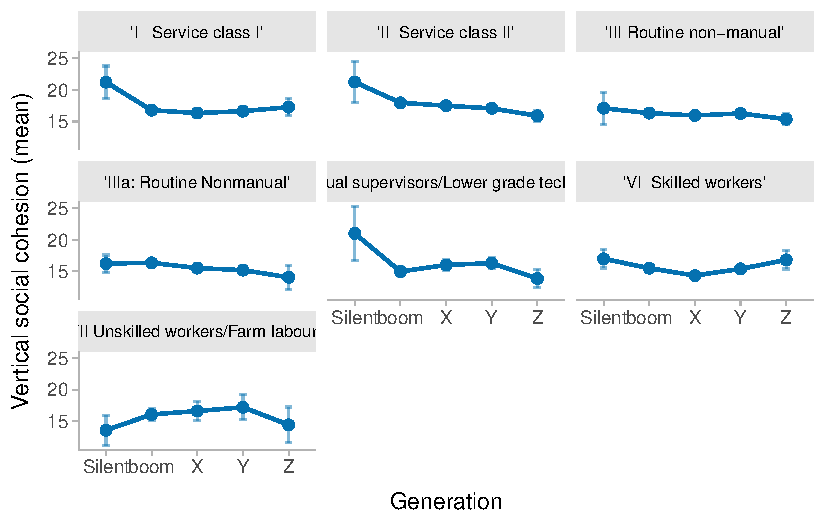
\includegraphics[keepaspectratio]{05-resultados_files/figure-pdf/fig-bivariado-1.pdf}}

}

\end{figure}%

La Figura~\ref{fig-bivariado} presenta un análisis bivariado que examina
la media de la cohesión social vertical (eje Y) a través de cinco
cohortes generacionales (Generation: Silent, Boom, X, Y, Z, en el eje
X), segmentado o facetado por las distintas categorías del esquema de
clase social EGP-7. Las barras verticales alrededor de cada punto
representan los intervalos de confianza al 95\%, lo que permite evaluar
la precisión de las estimaciones y la significancia visual de las
diferencias.

En primer lugar, se observa un efecto generacional parcialmente
consistente con la hipótesis H1, caracterizado por una tendencia
descendente de la cohesión social vertical a medida que las cohortes son
más jóvenes (de Silent hacia Z). Este patrón de ``caída'' generacional
es especialmente pronunciado y nítido en las clases socioeconómicas más
altas, como Service Class I y Service Class II, así como en las
ocupaciones de rutina no manuales (Routine non-manual y Routine
Nonmanual IIIa), donde los miembros de la generación Silent reportan
niveles de cohesión significativamente más altos (superando los 20
puntos en las clases de servicios) en comparación con las generaciones
sucesivas, las cuales tienden a estancarse o seguir descendiendo
sutilmente en torno a los 15-17 puntos.

En segundo lugar, el comportamiento de las clases manuales y
trabajadoras (EGP-V, VI y VII) quiebra la linealidad del descenso
generacional, mostrando dinámicas heterogéneas. En la categoría V
(Manual supervisors/Lower grade technicians) se aprecia un desplome
drástico entre la generación Silent y los Boomers, seguido de una leve
recuperación en las generaciones intermedias antes de volver a caer en
la generación Z. Por otro lado, la clase VI (Skilled workers) exhibe un
patrón en forma de ``U'': la cohesión disminuye desde la generación
Silent hasta alcanzar su punto más bajo en la Generación X, para luego
experimentar un repunte sistemático y estadísticamente visible en las
generaciones más jóvenes (Y y Z). Una tendencia inversa o de curva
invertida se observa en la clase VII (Unskilled workers/Farm labours),
donde la generación Silent inicia con los niveles de cohesión más bajos
(cercanos a 13 puntos), sube de forma sostenida hacia las generaciones
Boomer, X e Y, y vuelve a contraerse con la llegada de la generación Z.

En tercer lugar, el análisis de los intervalos de confianza revela un
problema de densidad de datos en los extremos generacionales dentro de
ciertas clases. Las barras de error para la generación Silent en casi
todos los paneles---y para la generación Z en categorías específicas
como la clase VII o la categoría ``NA''---son notablemente más amplias.
Esto coincide con el reporte descriptivo previo, confirmando que al
desagregar la muestra por celdas específicas (como Silent en la clase
VII), el tamaño muestral (n) se reduce sustancialmente, lo que disminuye
la precisión de la estimación bivariada e incrementa la incertidumbre en
los márgenes de error.

\begin{Shaded}
\begin{Highlighting}[]
\NormalTok{data\_f }\SpecialCharTok{\%\textgreater{}\%}
  \FunctionTok{ggplot}\NormalTok{(}\FunctionTok{aes}\NormalTok{(}\AttributeTok{x =}\NormalTok{ Generacion, }\AttributeTok{y =}\NormalTok{ c05\_total, }\AttributeTok{fill =}\NormalTok{ Generacion)) }\SpecialCharTok{+}
  \FunctionTok{geom\_violin}\NormalTok{(}\AttributeTok{alpha =}\NormalTok{ .}\DecValTok{6}\NormalTok{) }\SpecialCharTok{+}
  \FunctionTok{geom\_boxplot}\NormalTok{(}\AttributeTok{width =}\NormalTok{ .}\DecValTok{2}\NormalTok{, }\AttributeTok{alpha =}\NormalTok{ .}\DecValTok{8}\NormalTok{) }\SpecialCharTok{+}
  \FunctionTok{scale\_fill\_manual}\NormalTok{(}\AttributeTok{values =} \FunctionTok{c}\NormalTok{(}\StringTok{"\#0571B0"}\NormalTok{,}\StringTok{"\#92C5DE"}\NormalTok{,}\StringTok{"\#b3b3b3ff"}\NormalTok{,}\StringTok{"\#F4A582"}\NormalTok{,}\StringTok{"\#CA0020"}\NormalTok{)) }\SpecialCharTok{+}
  \FunctionTok{labs}\NormalTok{(}\AttributeTok{x =} \ConstantTok{NULL}\NormalTok{, }\AttributeTok{y =} \StringTok{"Cohesión social vertical"}\NormalTok{,}
       \AttributeTok{caption =} \StringTok{"Source: ELSOC 2016{-}2023"}\NormalTok{) }\SpecialCharTok{+}
  \FunctionTok{theme\_ggdist}\NormalTok{() }\SpecialCharTok{+}
  \FunctionTok{theme}\NormalTok{(}\AttributeTok{legend.position =} \StringTok{"none"}\NormalTok{)}
\end{Highlighting}
\end{Shaded}

\pandocbounded{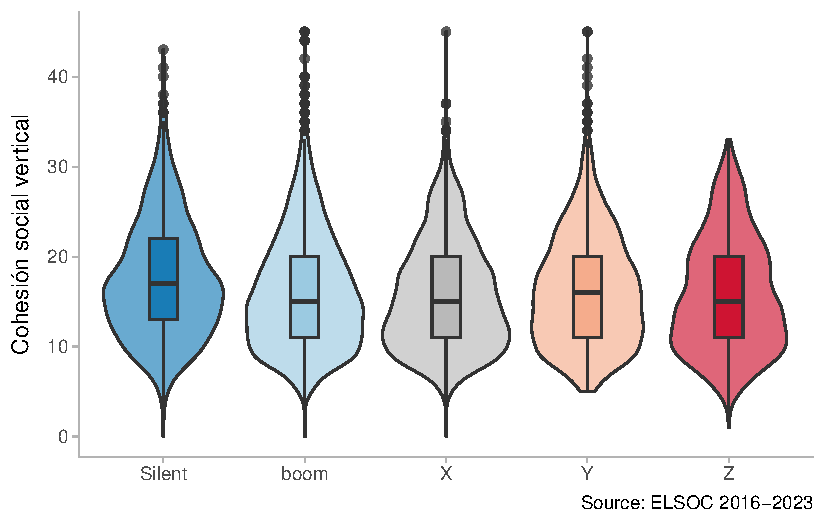
\includegraphics[keepaspectratio]{05-resultados_files/figure-pdf/unnamed-chunk-2-1.pdf}}

respecto a la tendencia central y la hipótesis H1, las cajas internas
muestran un descenso progresivo en las medianas conforme nos desplazamos
de las generaciones mayores a las más jóvenes. La generación Silent
exhibe la mediana más alta (en torno a los 17 puntos), mientras que las
generaciones Boomer, X, Y y Z muestran un estancamiento en sus medianas,
estabilizándose de forma muy similar alrededor de los 15 puntos. Este
comportamiento apoya parcialmente la idea de que las cohortes más
jóvenes muestran un menor apego o evaluación de la cohesión vertical en
comparación con la cohorte histórica de mayor edad, aunque la diferencia
se mitiga sustancialmente entre los bloques de las cuatro generaciones
sucesivas.

En segundo lugar, el análisis de la densidad (forma del violín)
demuestra una alta homogeneidad estructural. Todos los violines exhiben
una forma de ``diamante'' o distribución unimodal simétrica,
ensanchándose notoriamente en la franja de los 12 a los 20 puntos. Esto
indica que independientemente de la generación a la que pertenezca el
individuo, la gran mayoría de la población tiende a concentrar sus
respuestas en valores moderados-bajos de cohesión social vertical. No se
aprecian distribuciones bimodales (que sugerirían una polarización
extrema de opiniones dentro de una misma generación), sino un consenso
generalizado en torno al centro-inferior de la escala.

Modelos de regresion.

{

\begin{longtable}[]{@{}llllll@{}}

\caption{\label{tbl-modelos}Multilevel models for vertical social
cohesion}

\tabularnewline

\toprule\noalign{}
~ & Modelo 0 & Modelo Temp. & Modelo 1 & Modelo 3 & Modelo 4 \\
\midrule\noalign{}
\endhead
\midrule\noalign{}
\multicolumn{6}{@{}l@{}}{%
Note: Cells contain regression coefficients with standard errors in
parentheses. \textsuperscript{***}p \textless{} 0.001;
\textsuperscript{**}p \textless{} 0.01; \textsuperscript{*}p \textless{}
0.05.} \\
\bottomrule\noalign{}
\endlastfoot
Intercept & 15.848\textsuperscript{***} & 15.711\textsuperscript{***} &
15.899\textsuperscript{***} & 21.493\textsuperscript{***} &
21.303\textsuperscript{***} \\
~ & (0.111) & (0.180) & (0.106) & (2.298) & (2.297) \\
Corruption perception (Grand-mean centered) & ~ & ~ &
-0.789\textsuperscript{***} & -0.480\textsuperscript{***} &
-0.494\textsuperscript{***} \\
~ & ~ & ~ & (0.081) & (0.075) & (0.077) \\
Corruption perception (Person historical mean) & ~ & ~ & ~ &
-1.599\textsuperscript{***} & -1.596\textsuperscript{***} \\
~ & ~ & ~ & ~ & (0.180) & (0.180) \\
Age (Specific-mean centered) & ~ & ~ & 0.075\textsuperscript{**} & 0.030
& -0.053 \\
~ & ~ & ~ & (0.028) & (0.045) & (0.078) \\
Age (Person historical mean) & ~ & ~ & ~ & 0.012 & 0.014 \\
~ & ~ & ~ & ~ & (0.022) & (0.022) \\
National identification (Grand-mean centered) & ~ & ~ &
0.733\textsuperscript{***} & 0.341\textsuperscript{***} &
0.340\textsuperscript{***} \\
~ & ~ & ~ & (0.090) & (0.083) & (0.083) \\
National identification (Person historical mean) & ~ & ~ & ~ &
0.819\textsuperscript{***} & 0.822\textsuperscript{***} \\
~ & ~ & ~ & ~ & (0.213) & (0.212) \\
Dignified treatment (Grand-mean centered) & ~ & ~ & ~ &
-0.062\textsuperscript{**} & -0.055\textsuperscript{**} \\
~ & ~ & ~ & ~ & (0.021) & (0.021) \\
Dignified treatment (Specific-mean centered) & ~ & ~ &
0.164\textsuperscript{***} & ~ & ~ \\
~ & ~ & ~ & (0.016) & ~ & ~ \\
Dignified treatment (Person historical mean) & ~ & ~ & ~ &
-0.111\textsuperscript{**} & -0.144\textsuperscript{***} \\
~ & ~ & ~ & ~ & (0.037) & (0.038) \\
Political self-identification (Grand-mean centered) & ~ & ~ &
-0.090\textsuperscript{***} & -0.111\textsuperscript{***} &
-0.108\textsuperscript{***} \\
~ & ~ & ~ & (0.018) & (0.017) & (0.017) \\
Political self-identification (Person historical mean) & ~ & ~ & ~ &
-0.182\textsuperscript{***} & -0.189\textsuperscript{***} \\
~ & ~ & ~ & ~ & (0.041) & (0.041) \\
Sex: Female & ~ & ~ & ~ & -0.067 & -0.094 \\
~ & ~ & ~ & ~ & (0.195) & (0.196) \\
Education: Basic & ~ & ~ & ~ & 0.659 & 0.707 \\
~ & ~ & ~ & ~ & (0.873) & (0.861) \\
Education: Higher education & ~ & ~ & ~ & 1.658 & 1.698 \\
~ & ~ & ~ & ~ & (0.888) & (0.876) \\
Education: Postgraduate & ~ & ~ & ~ & 2.909\textsuperscript{**} &
2.969\textsuperscript{**} \\
~ & ~ & ~ & ~ & (1.001) & (0.991) \\
Generation: Boom & ~ & ~ & ~ & -1.074 & -1.068 \\
~ & ~ & ~ & ~ & (0.689) & (0.688) \\
Generation: X & ~ & ~ & ~ & -1.337 & -1.327 \\
~ & ~ & ~ & ~ & (0.883) & (0.882) \\
Generation: Y & ~ & ~ & ~ & -1.089 & -1.052 \\
~ & ~ & ~ & ~ & (1.093) & (1.092) \\
Generation: Z & ~ & ~ & ~ & -1.524 & -1.481 \\
~ & ~ & ~ & ~ & (1.309) & (1.308) \\
Intermediate class (III+IV) & ~ & ~ & ~ & -0.419\textsuperscript{*} &
-0.426\textsuperscript{*} \\
~ & ~ & ~ & ~ & (0.178) & (0.181) \\
Working class (V+VI+VII) & ~ & ~ & ~ & -0.812\textsuperscript{***} &
-0.864\textsuperscript{***} \\
~ & ~ & ~ & ~ & (0.190) & (0.194) \\
Wave 2017 & ~ & 2.113\textsuperscript{***} & ~ &
1.409\textsuperscript{***} & 1.526\textsuperscript{***} \\
~ & ~ & (0.210) & ~ & (0.292) & (0.292) \\
Wave 2018 & ~ & 3.719\textsuperscript{***} & ~ &
3.463\textsuperscript{***} & 3.539\textsuperscript{***} \\
~ & ~ & (0.195) & ~ & (0.223) & (0.257) \\
Wave 2019 & ~ & -1.800\textsuperscript{***} & ~ &
-2.319\textsuperscript{***} & -2.090\textsuperscript{***} \\
~ & ~ & (0.194) & ~ & (0.307) & (0.367) \\
Wave 2021 & ~ & -4.866\textsuperscript{***} & ~ &
-5.585\textsuperscript{***} & -5.279\textsuperscript{***} \\
~ & ~ & (0.195) & ~ & (0.332) & (0.428) \\
Wave 2022 & ~ & 0.712\textsuperscript{***} & ~ & 0.053 & 0.516 \\
~ & ~ & (0.195) & ~ & (0.383) & (0.541) \\
Wave 2023 & ~ & 3.043\textsuperscript{***} & ~ &
2.242\textsuperscript{***} & 2.642\textsuperscript{***} \\
~ & ~ & (0.210) & ~ & (0.418) & (0.591) \\
BIC & 51120.934 & 48412.698 & 50880.197 & 48179.382 & 48144.670 \\
Num. obs. & 7979 & 7979 & 7979 & 7979 & 7979 \\
Num. groups: individuals & 1372 & 1372 & 1372 & 1372 & 1372 \\
Var: individuals (Intercept) & 11.697 & 12.197 & 10.330 & 8.650 &
8.804 \\
Var: individuals (Age within) & 28.789 & 19.238 & 28.027 & 18.991 &
17.772 \\
Cov: individuals (Intercept - Age within) & ~ & ~ & ~ & ~ & 0.195 \\
Var: Residual & ~ & ~ & ~ & ~ & -0.091 \\

\end{longtable}

}

El análisis comenzó mediante la estimación de un Modelo Nulo o de
intercepto aleatorio (Modelo 0). Este paso inicial resultó fundamental
para ejecutar la partición de la varianza y calcular el Coeficiente de
Correlación Intraclase (ICC), determinando así si la estructura anidada
de los datos, donde las observaciones longitudinales se encuentran
agrupadas dentro de los mismos individuos, requería un tratamiento
estadístico jerárquico. Los resultados del Modelo 0 revelaron una
varianza entre individuos (\(\tau_{00}\)) de 11.697 en el Nivel 2 y una
varianza residual (\(\sigma^2\)) de 28.789 en el Nivel 1. A partir de
estos componentes, el cálculo del ICC arrojó un valor de 0.289, lo que
indica que el 28.9\% de la variabilidad total de la confianza
institucional es explicada por diferencias estables y basales entre las
personas (efectos \emph{between-individual}), mientras que el 71.1\%
restante responde a fluctuaciones temporales dentro del individuo a lo
largo del tiempo o a errores de medición (efectos
\emph{within-individual}). Dado que este coeficiente supera ampliamente
el umbral crítico del 10\% sugerido por la literatura, se justifica
técnicamente el uso de modelos de efectos mixtos para corregir la no
independencia de las observaciones y evitar sesgos en la estimación del
error estándar.

Posterior y progresivamente, la especificación de los siguientes modelos
incorporó variables de percepción y atributos sociodemográficos fijos,
permitiendo identificar con precisión los factores estructurales y
subjetivos que movilizan la dimensión vertical en el país. Dentro de las
variables, la percepción de corrupción centrado en la gran media
(\emph{Grand-mean centered}) emergió como un inhibidor crítico del
modelo (Modelo 1, \(\beta = -0.789, p < 0.001\)), aportando evidencia
empírica a favor de la hipótesis de que la sospecha de corrupción
erosiona de raíz la legitimidad del vínculo jerárquico que une a la
sociedad con el Estado. En contraposición a este efecto erosivo, la
identificación nacional bajo este mismo centrado funcionó como un
habilitador positivo de particular relevancia
(\(\beta = 0.733, p < 0.001\)), respaldando la premisa de que la
identidad nacional opera como un ``amortiguador'' o reserva cultural que
estabiliza la percepción del orden social incluso frente a escenarios de
profunda desafección institucional. Esta dinámica de opiniones se
encuentra fuertemente condicionada por la posición objetiva de los
sujetos en la estructura social, manifestada a través de la educación y
la clase social. Al evaluar el esquema colapsado, la clase trabajadora
manual exhibe niveles significativamente menores de confianza vertical
en comparación con la clase de servicios (Modelo 3,
\(\beta = -0.812, p < 0.001\)), un hallazgo que delata cómo la
heterogeneidad estructural del mercado laboral chileno y la exclusión de
los beneficios del desarrollo se traducen en un distanciamiento del
pacto social, patrón que también afecta de forma significativa a la
clase intermedia (\(\beta = -0.419, p < 0.05\)). Asimismo, el rol de la
educación no se comporta de manera lineal; el modelo demuestra que solo
el nivel de posgrado actúa como un dinamizador positivo y robusto en
comparación con la categoría de referencia
(\(\beta = 2.909, p < 0.01\)), sugiriendo que la alta especialización
académica facilita una inserción privilegiada en las jerarquías del país
y, por ende, una evaluación más favorable de las mismas.

Por otra parte, los modelos capturan una fractura generacional basal
combinada con la vulnerabilidad del sistema ante los acontecimientos
históricos recientes. Al analizar las cohortes, y a pesar de la pérdida
de significancia estadística por el control multivariado, la Generación
Z registra el coeficiente negativo más pronunciado en la estructura
generacional (\(\beta = -1.524\) en Modelo 3), delineando una tendencia
al alejamiento del orden institucional por parte de los ciudadanos más
jóvenes en comparación con la generación \emph{Silent}. Este
distanciamiento coexistió con un fuerte shock de contexto capturado a
través de las variables temporales de Ola. Específicamente, se observa
una caída estrepitosa en la Ola 5, correspondiente al año 2021 (Modelo
3, \(\beta = -5.585, p < 0.001\)), la cual refleja de manera nítida el
impacto acumulado del Estallido Social de 2019 y las disrupciones
socioeconómicas de la pandemia del COVID-19 en la degradación del tejido
institucional del país, mostrando un proceso de recuperación hacia la
Ola 2023 (\(\beta = 2.242, p < 0.001\)).

Siguiendo la necesidad de modelar la heterogeneidad de las respuestas
individuales, el Modelo 4 fue enriquecido mediante la inclusión de una
pendiente aleatoria para la edad centrada en el promedio de la persona
(\emph{Age specific-mean centered}). El valor 0.195 corresponde a la
covarianza entre el intercepto y la pendiente, y la consecuente
reducción en el Criterio de Información Bayesiano (BIC) de 48179.38 a
48144.67 son evidencia a favor de que el paso del tiempo y el
envejecimiento intraindividual no afectan a todos los chilenos por
igual.

Finalmente, el Modelo 4 se consolidó como la especificación
metodológicamente superior al presentar el mejor ajuste general, cuya
virtud principal radica en su capacidad para desagregar los componentes
inter e intraindividuales a través de dos estrategias distintas de
centrado. Para las variables de Percepción de Corrupción, Identificación
Nacional y Autoidentificación Política, el modelo emplea un centrado en
la gran media (\emph{Grand-mean centered}) en el Nivel 1 en coexistencia
con el promedio histórico del sujeto (\emph{Person historical mean}) en
el Nivel 2. Bajo esta formulación algebraica, el promedio histórico
absorbe la varianza interindividual total, forzando a los coeficientes
de Nivel 1 a transformarse en efectos \emph{Within} puros
(intraindividuales), mientras que los coeficientes de las medias
históricas en el Nivel 2 deben interpretarse estrictamente como
\textbf{efectos contextuales netos} (\(\beta_B - \beta_W\)). A través de
esta descomposición, se constató que el efecto contextual de la
cronicidad de la corrupción (\(\beta = -1.596, p < 0.001\)) es más de
tres veces superior a su fluctuación anual momentánea
(\(\beta = -0.494, p < 0.001\)). Esto demuestra que para dos
observaciones con el mismo nivel de percepción en un año dado, el
individuo que arrastra un historial crónico de sospecha institucional
sufre una penalización contextual severa en su confianza basal.
Homólogamente, el promedio histórico de la identificación nacional opera
como un potente efecto contextual positivo
(\(\beta = 0.822, p < 0.001\)) en comparación con su desvío anual
(\(\beta = 0.340, p < 0.001\)). Por el contrario, para las variables de
Edad y Trato Digno se optó por un centrado en la media del sujeto
(\emph{Specific-mean centered}) en el Nivel 1. Esta estrategia
metodológica separa de manera directa los paramétrod: el término
centrado arroja el efecto \emph{Within} puro, mientras que la media
histórica en el Nivel 2 provee directamente el \textbf{efecto
\emph{Between} puro} (\(\beta_B\)).El análisis del Trato Digno en el
Modelo 3 ilustra una sugerente paradoja; por un lado, el incremento
coyuntural del trato digno respecto al propio promedio del sujeto eleva
significativamente su confianza institucional
(\(\beta = 0.164, p < 0.001\), efecto Within). Por otro lado, el efecto
Between revela una dinámica contraintuitiva; aquellos individuos con
trayectorias estables de mayor trato digno en el tiempo exhiben una
menor confianza institucional (\(\beta = -0.111, p < 0.01\)).

Al contrastar el cuerpo de hipótesis con las estimaciones de los
modelos, se observa un respaldo empírico parcial para las principales
tesis del estudio. Se halla evidencia concluyente a favor de la
Hipótesis 3 (Identificación nacional), dado que tanto el coeficiente de
variación temporal (\(\beta = 0.340, p < 0.001\)) como, muy
especialmente, el efecto del historial crónico interindividual del
sujeto (\(\beta = 0.822, p < 0.001\)) son significativos, directos y
positivos. De igual forma, existe sustento empírico sólido para la
Hipótesis 5 (Variación temporal macro-contingente), confirmándose que
las crisis político-sanitarias de la Ola 2019
(\(\beta = -2.090, p < 0.001\)) y la Ola 2021
(\(\beta = -5.279, p < 0.001\)) contrajeron de forma estrepitosa el
constructo dependiente, aunque la Ola 2022 perdió significancia al
controlar por efectos interindividuales en el Modelo 4
(\(\beta = 0.516\)). Por el contrario, la Hipótesis 1 (Cohorte
generacional) es rechazada debido a que ninguna de las cohortes alcanzó
significancia estadística frente a la generación \emph{Silent}
(registrando la Generación Z un \(\beta = -1.481\) no significativo en
el Modelo 4), descartándose un alejamiento generacional neto una vez
controladas las variables de percepción. La Hipótesis 2 (Clase social)
sufre una contradicción de signo fundamental; aunque se hipotetizaba un
efecto positivo (\(\gamma^{\text{EGP}}_{40} > 0\)), la clase trabajadora
manual exhibió un coeficiente significativamente negativo
(\(\beta = -0.864, p < 0.001\)), lo que demuestra que pertenecer a estos
estratos debilita la confianza institucional en lugar de fortalecerla.
Respecto al capital educativo (Hipótesis 4), el supuesto de un
incremento monótono se descarta, puesto que solo el nivel de posgrado
demostró un efecto dinamizador y estadísticamente significativo
(\(\beta = 2.969, p < 0.01\)) en comparación con la categoría de base.
Finalmente, la Hipótesis 6 (Moderación de la trayectoria temporal)
carece de soporte empírico en la especificación actual, dado que las
dinámicas contractivas observadas en el tiempo operaron como shocks
paralelos y transversales a la estructura de las cohortes, sin mostrar
interacciones cruzadas estadísticamente significativas que permitiesen
validar una penalización asimétrica en la juventud.

\bookmarksetup{startatroot}

\chapter{Conclusiones}\label{conclusiones}

La discusión de los hallazgos empíricos a la luz de la literatura
especializada permite desentrañar la compleja y precaria configuración
de la dimensión vertical de la cohesión social en Chile, tomando como
eje vertebrador la confianza en las instituciones. Teóricamente, este
constructo es entendido como el ``pegamento social'' que regula el
vínculo jerárquico entre la ciudadanía y el aparato estatal, actuando
como un pilar indispensable para sostener la estabilidad democrática y
dinamizar el desarrollo inclusivo
(\citeproc{ref-chan_charting_2006}{Chan \& Chan, 2006};
\citeproc{ref-kim_social_2021}{Kim et~al., 2021}). No obstante, la
evidencia longitudinal provista por este estudio revela que dicho
pegamento estructural se encuentra críticamente debilitado en el
escenario nacional. El hecho de que el Modelo 0 registre que un 71.1\%
de la varianza total responda a fluctuaciones temporales
intraindividuales da cuenta de una profunda volatilidad y desafección,
lo que sintoniza con el diagnóstico del Ministerio de Desarrollo Social
y Familia
(\citeproc{ref-ministeriodedesarrollosocialyfamilia_informe_2020}{Ministerio
de Desarrollo Social y Familia, 2020}) respecto a que las organizaciones
fundamentales del régimen político chileno exhiben índices de confianza
residuales situados de manera persistente por debajo del umbral del 5\%.

Esta erosión sistémica encuentra su explicación teórica más robusta en
el impacto destructivo de la corrupción y el rol moderador de los lazos
identitarios. Mientras autores como Han et al.
(\citeproc{ref-_essentials_2017}{{«({PDF}) {The Essentials} of {Social
Cohesion}»}, 2017}) sostienen que la integridad y la justicia percibida
en la praxis gubernamental son precondiciones esenciales para la
validación pública del orden social, los resultados de la descomposición
híbrida del Modelo 4 identifican a la percepción de corrupción crónica
como el inhibidor más potente de la confianza
(\(\beta = -1.596, p < 0.001\)). El hallazgo de que el promedio
histórico de corrupción de un sujeto (\emph{Person historical mean})
posea un peso predictivo tres veces superior a su fluctuación anual
momentánea corrobora que la legitimidad en Chile no es vulnerable a
escándalos coyunturales o aislados, sino que arrastra el costo de una
desconfianza crónica acumulada que destruye de manera sistémica la
credibilidad del Estado (\citeproc{ref-kim_social_2021}{Kim et~al.,
2021};
\citeproc{ref-ministeriodedesarrollosocialyfamilia_informe_2020}{Ministerio
de Desarrollo Social y Familia, 2020}). Frente a este panorama
contractivo, el análisis valida la perspectiva de Schiefer y van der
Noll (\citeproc{ref-__essentials_2017}{\textbf{\_\_essentials\_2017?}}),
para quienes la identificación con la unidad geográfica es una dimensión
esencial de la resiliencia social; en efecto, el sentimiento de
identificación nacional estable y basal del individuo se erige en el
principal dinamizador del modelo (\(\beta = 0.822, p < 0.001\)),
operando como una suerte de ``reserva cultural'' o amortiguador
subjetivo que sostiene el apego cívico mínimo hacia el orden social
incluso cuando las agencias políticas atraviesan su peor crisis de
legitimidad
(\citeproc{ref-__cohesion_2022}{\textbf{\_\_cohesion\_2022?}}).

Por otra parte, al examinar las coordenadas sociodemográficas, el rol de
la estratificación socioeconómica y la edad revela profundas brechas en
la integración al pacto social. Los datos chilenos contradicen
parcialmente la tesis internacional de Kim et al.
(\citeproc{ref-kim_social_2021}{Kim et~al., 2021}), quienes asumen que
las clases altas confían menos debido a estándares normativos más
severos en la evaluación del desempeño estatal. Por el contrario, en el
contexto nacional es la clase trabajadora manual (\(\text{V+VI+VII}\))
la que manifiesta los niveles significativamente más bajos de confianza
vertical (\(\beta = -0.864, p < 0.001\)), lo que se explica de mejor
manera bajo el prisma de la heterogeneidad estructural latinoamericana
propuesto por Molina y Alfageme
(\citeproc{ref-molina_repensando_2022}{Molina \& Alfageme, 2022}), donde
la exclusión histórica de los beneficios del desarrollo económico y la
precariedad laboral endémica producen un distanciamiento material y
subjetivo de las estructuras reguladoras. Esta asimetría estructural
coexiste con una notable fractura generacional que desafía el clásico
supuesto de continuidad histórica; la marcada tendencia negativa
observada en la Generación Z (\(\beta = -1.524\) en el Modelo 3) sugiere
que las cohortes más jóvenes en Chile han salido de lo que Heidegger
conceptualiza como el ``surco trazado por el tiempo''
(\citeproc{ref-diazsarmiento_entendiendo_2017}{Díaz Sarmiento et~al.,
2017}), rompiendo la inercia institucional que caracterizaba a
generaciones precedentes ---como la generación \emph{Silent} o los
\emph{Boomers}--- para situarse en un perfil de ciudadanía altamente
movilizada pero profundamente desconfiada de las jerarquías
tradicionales del Estado
(\citeproc{ref-__cohesion_2022}{\textbf{\_\_cohesion\_2022?}}).

Finalmente, esta fragilidad multidimensional se vio críticamente
tensionada por shocks externos de gran envergadura que aceleraron el
desanclaje institucional. La caída estrepitosa en la confianza vertical
registrada durante la Ola 2021 (\(\beta = -5.585, p < 0.001\)) captura
nítidamente el impacto acumulado del Estallido Social de 2019 y las
disrupciones socioeconómicas de la pandemia por COVID-19. Estos
acontecimientos operaron como coyunturas críticas que pusieron a prueba
la capacidad de respuesta, eficacia y protección del Estado, cuya
evaluación deficiente por parte de la ciudadanía terminó por fracturar
el tejido institucional y profundizar la desafección vertical
(\citeproc{ref-ministeriodedesarrollosocialyfamilia_informe_2020}{Ministerio
de Desarrollo Social y Familia, 2020};
\citeproc{ref-han2021}{\textbf{han2021?}}). En suma, la dimensión
vertical en Chile se define hoy como un equilibrio precario e inestable
donde la identidad nacional sostiene artificialmente el andamiaje del
sistema, mientras que la percepción crónica de corrupción, la exclusión
estructural de las clases manuales y la desafección radical de las
nuevas generaciones actúan como fuerzas inhibidoras de fondo que los
shocks exógenos de corto plazo terminan por agravar de manera crítica.

\bookmarksetup{startatroot}

\chapter{Referencias}\label{referencias}

\cleardoublepage
\phantomsection
\addcontentsline{toc}{part}{Apéndices}
\appendix

\chapter{Instrumentos de
levantamiento}\label{instrumentos-de-levantamiento}

Incluye cuestionarios, guias de entrevista, etc.

\chapter{Tablas adicionales}\label{tablas-adicionales}

Tablas extendidas, tests de robustez, etc.

\protect\phantomsection\label{refs}
\begin{CSLReferences}{1}{0}
\bibitem[\citeproctext]{ref-chan_charting_2006}
Chan, J., \& Chan, E. (2006). Charting the {State} of {Social Cohesion}
in {Hong Kong}. \emph{The China Quarterly}, \emph{187}, 635-658.
\url{https://doi.org/10.1017/S0305741006000415}

\bibitem[\citeproctext]{ref-_cohesion_2022}
\emph{{Cohesión social en Chile en tiempos de cambio: indicadores,
perfiles y factores asociados \textbar{} CEPAL}}. (2022).
https://www.cepal.org/es/publicaciones/47735-cohesion-social-chile-tiempos-cambio-indicadores-perfiles-factores-asociados.

\bibitem[\citeproctext]{ref-diazsarmiento_entendiendo_2017}
Díaz Sarmiento, C., López Lambraño, M., \& Roncallo Lafont, L. (2017).
{Entendiendo las generaciones: una revisión del concepto, clasificación
y características distintivas de los Baby Boomers, X Y Millennials}.
\emph{CLIO América}, \emph{11}(22 (Julio - Diciembre)), 188-204.

\bibitem[\citeproctext]{ref-han_trust_2021}
Han, Q., Zheng, B., Cristea, M., Agostini, M., \& Et., A. (2021). Trust
in Government Regarding {COVID-19} and Its Associations with Preventive
Health Behaviour and Prosocial Behaviour during the Pandemic: A
Cross-Sectional and Longitudinal Study. \emph{Psychological Medicine}.
\url{https://doi.org/10.1017/s0033291721001306}

\bibitem[\citeproctext]{ref-kim_social_2021}
Kim, Y., Sommet, N., Na, J., \& Spini, D. (2021). Social {Class}---{Not
Income Inequality}---{Predicts Social} and {Institutional Trust}.
\emph{Social Psychological and Personality Science}, \emph{13},
194855062199927. \url{https://doi.org/10.1177/1948550621999272}

\bibitem[\citeproctext]{ref-_confianza_2024}
{La confianza en las instituciones públicas de Chile: Los determinantes
de la confianza en las instituciones públicas de Chile}. (2024). En
\emph{OECD}.
https://www.oecd.org/es/publications/los-determinantes-de-la-confianza-en-las-instituciones-publicas-de-chile\_9cdf8865-es/full-report/component-5.html.

\bibitem[\citeproctext]{ref-ministeriodedesarrollosocialyfamilia_informe_2020}
Ministerio de Desarrollo Social y Familia. (2020). \emph{Informe Final
{Consejo Asesor} Para La {Cohesión Social}}. Ministerio de Desarrollo
Social y Familia.

\bibitem[\citeproctext]{ref-molina_repensando_2022}
Molina, E. C., \& Alfageme, C. (2022). {Repensando la estructura de
clases en formato comparativo en el marco de los procesos de
heterogeneidad del mercado laboral en América Latina y Europa1}.
\emph{EMPIRIA. Revista de Metodología de las Ciencias Sociales},
\emph{55}, 155-178.

\bibitem[\citeproctext]{ref-silveira_mixedeffects_2023}
Silveira, L. T. Y. da, Ferreira, J. C., \& Patino, C. M. (2023).
{Mixed-effects model: a useful statistical tool for longitudinal and
cluster studies}. \emph{Jornal Brasileiro De Pneumologia: Publicacao
Oficial Da Sociedade Brasileira De Pneumologia E Tisilogia},
\emph{49}(2), e20230137.
\url{https://doi.org/10.36416/1806-3756/e20230137}

\bibitem[\citeproctext]{ref-_essentials_2017}
The {Essentials} of {Social Cohesion}: {A Literature Review}. (2017).
\emph{ResearchGate}. \url{https://doi.org/10.1007/s11205-016-1314-5}

\end{CSLReferences}


\backmatter

% --- Cuerpo del libro (capítulos) en arábigos ---
\mainmatter
\pagestyle{scrheadings}

% --- (Opcional) Estilo del índice general ---
% \addtocontents{toc}{\protect\thispagestyle{plain}}


\end{document}
